\section{Clase 7}
\begin{defi}
	Una estructura $(A,+,\cdot)$ es una anillo si
	\begin{itemize}
		\item $(A,+)$ es un grupo abeliano
		\item $(A,\cdot)$ es un semigrupo
	\end{itemize}
\end{defi}

En el caso que la operación de multiplicación admita un elemento unidad, entonces \anillo será un anillo con unidad, i.e. $\forall x\in A, \exists x\in A / ex=xe=x$.

En el caso que la operación multiplicativa del anillo sea conmutativa, el anillo es un anillo conmutativo.

\begin{defi}
	Un campo denotado por $K$, es una estructura que además de tener las propiedades del anillo con unidad, cada elemento $A$, excepto el cero, tiene un inverso. Por lo tanto un campo \campo es una estructura tal que
	\begin{itemize}
		\item $(K,+)$ es un grupo abeliano aditivo.
		\item $(K-0, \cdot)$ es un grupo abeliano multiplciativo.
	\end{itemize}
\end{defi}

Hasta ahora hemos estudiado estructuras que tienen una ó dos operaciones binarias internas. Consideremos ahora una estructura dotada de una operación binaria interna y una operación binaria externa.

\subsection{Espacio lineal o espacio vectorial}
\begin{defi}
	Una estructura \espvec es llamado un espacio vectorial, si
	\begin{itemize}
		\item $M$ es un grupo abeliano,
		\item $K$ es un campo conmutativo,
		\item $\bullet$ es una operación binaria externa que define la acción del campo $K$ sobre el grupo $M$,
		\begin{align}
  \bullet &:K\times M\to M\\
  &(\alpha,x)\to \alpha \bullet x,\qquad\forall x\in M, \forall\alpha\in K
\end{align}
\item La operación binaria interna de $M$ está relacionada con la operación binaria externa $\bullet$ a través de una operación distintiva mixta. 
\begin{itemize}
	\item $\alpha \bullet (x+y)=\alpha\bullet x+\alpha\bullet y$
	\item $(\alpha + \beta)\bullet x = \alpha\bullet x+\beta\bullet y$
\end{itemize}
$\forall \alpha,\beta\in K,\forall x,y\in M$.
	\end{itemize}
\end{defi}

Normalmente los elementos $x\in M$ se llaman \textbf{vectores} y los elementos $\alpha\in K$ se llaman \textbf{escalares} y la operación $\bullet$ se llama producto por escalar.

\subsection{Álgebra y álgebra de Lie}
\begin{defi}
	Una estructura algebraica \algebra es llamada un álgebra, si
	\begin{itemize}
		\item $A$ es un anillo,
		\item $K$ es un campo conmutativo,
		\item $\bullet$ es una operación binaria externa que define la acción del campo $K$ sobre el anillo,
		\begin{equation}
  \bullet : K\times A\to A
\end{equation}
\item La operació binara interna aditiva del anillo $(+)$ está relacionada con la operación binaria externa a través de la propiedad distributiva mixta
\begin{itemize}
	\item $\a\bullet (x+y)=\a\bullet x\a\bullet y,\qquad \forall \a,\b \in K,\, \forall x,y\in A$
	\item $(\a +\b )x=\a\bullet x+\b\bullet x$
\end{itemize}
\item La operación binaria interna multiplicativa del anillo (denotada por $\diamond$) está relacionada con la operación binaria externa $\bullet$ por medio de la propiedad asociativa mixta
\begin{equation}
  \a\bullet(x\diamond y)=(\a\bullet x)\diamond y=x\diamond (\a\bullet y),\qquad \forall x,y\in A,\, \forall \a\in K
\end{equation}
	\end{itemize}
\end{defi}
\begin{enumerate}
\item La operación binaria interna del anillo $\diamond$ se le llama producto algebraico.

En el caso que la multiplicación algebraica $\diamond$ sea asociativa, i.e., $\forall x,y,z\in A$,
\begin{equation}
  (x\diamond y)\diamond z=x\diamond (y\diamond z)
\end{equation}
entonces el álgebra se llama \textbf{álgebra asociativa}.

\item Si la multiplicación algebraica tiene además de la propiedad asociativa, al elemento unidad entonces el álgebra es llamada \textbf{álgebra asociativa unital}.
\item Si la operación multiplicación algebraica es una operación antisimétrica, i.e., si
\item \begin{equation}
  x\diamond y=[x,y]=xy-yx
\end{equation}
entonces el álgebra se llama \textbf{álgebra de Lie} y la operación $\diamond$ antisimétrica satisface la propiedad derivativa conocida como identidad de Jacobi.
\end{enumerate}

\subsection{Grupos, álgebras y simetrías}
El concepto de grupo está muy relacionado con el concepto de invariancia o de simetría de objetos tales como superficies, funciones, ecuaciones algebraicas, ecuaciones diferenciales, entre otros.

\underline{\textbf{Nota histórica}: }
\begin{itemize}
	\item El estudio de las simetrías de las ecuaciones algebraicas se hace en el contexto de la teoría de Galois \footnote{\url{https://es.wikipedia.org/wiki/\%C3\%89variste_Galois}}.
	\item El estudio de las simetrías de las ecuaciones diferenciales se hacen en el contexto de la teoría de Lie \footnote{\url{https://es.wikipedia.org/wiki/Sophus_Lie}} .
\end{itemize}

Los grupos de Lie son grupos continuos que tienen la propiedad que es suficiente estudiarlos en su forma infinitesimal. En física, los grupos de Lie se introducen como grupos de transformaciones de coordenadas, i.e., como actuando sobre los elementos de una variedad.

\begin{ej}
Consideremos la típica rotación en un plano de los ejes coordenados en un ángulo $\th$,
	\begin{figure}[h!]
		\centering
		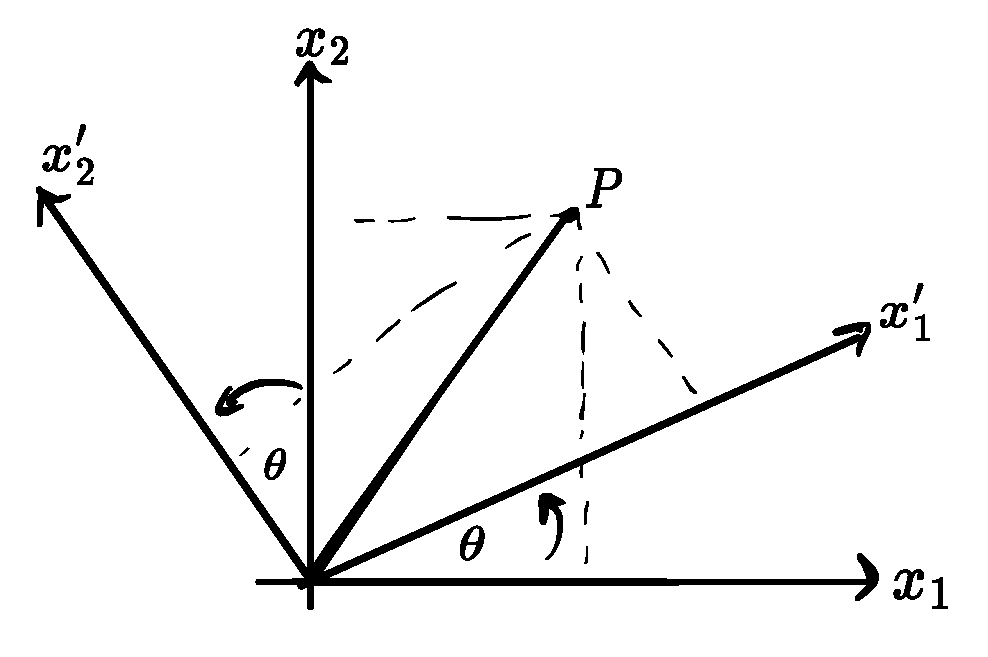
\includegraphics[scale=0.5]{sistema-coord.pdf}
%		\caption{Rotación en un plano.}
	\end{figure}
La relación entre las coordenadas primadas y las sin primar viene dada por
\begin{align}
  x'_1&=\cos\th x_1-\sin\th x_2\\
  x'_2&=\sin\th x_1+\cos\th x_2
\end{align}
o de manera equivalente
\begin{equation}
  \underbrace{\mqty(x_1'\\x'_2)}_{x'}=\underbrace{\mqty(\cos\th&-\sin\th\\\sin\th&\cos\th)}_{R(\th)}\underbrace{\mqty(x_1\\x_2)}_{x}
\end{equation}
Así, tenemos una transformación de la forma 
\begin{equation}
  x'=f(x,\th )
\end{equation}
además, notemos que 
\begin{itemize}
\item $\{R(\theta)\}$ tiene unidad $\forall \theta$, dada por
\begin{equation}
  R(0)=\mqty(1&0\\0&1)
\end{equation}
\item tiene inverso, $\forall\theta, \exists (-\theta)$.
\item es asociativo,
\item es conmutativo
\end{itemize}
Si la transformación $x'=f(x,\theta)$, entonces la unidad es dada por $x'=f(x,0)=f(x,e)=x$.
\end{ej}

\begin{defi}
	Un conjunto de transformaciones
	\begin{equation}
  x'^{i}=f^{i}(x',...,x^n;g^1,...,g^r)\equiv f(x,g)
\end{equation}
es llamado un \textbf{grupo de transformaciones $r$-paramétrico} si
\begin{enumerate}
	\item admite el elemento unidad
\begin{equation}
  x'=f(x,e)=x
\end{equation}
\item admite elemento inverso
\item tiene definida una ley de composición interna,
\begin{align}
  x'=f(x,g),\qquad x''=f(x',g')=f[f(x,g),g']=f(x,g'')
\end{align}
entonces 
\begin{equation}
  \boxed{g''=g''(g,g')}
\end{equation}
\end{enumerate}
\end{defi}
%
\begin{defi}
	Un conjunto de transformaciones es un \textbf{grupo de simetría} de una ecuación diferencial
	\begin{equation}\label{7.1}
  F(x,x^{(1)},...,x^{(n)})=0,\quad \text{con }x=(x^1,...,x^n)
\end{equation}
si la ecuación \eqref{7.1} permanece invariante en forma bajo la acción del grupo,
\begin{equation}
  F(x',x'^{(1)},...,x'^{(n)})=0
\end{equation}
\end{defi}

Lo interesante de los grupos de Lie es que basta estudiar sus versiones infinitesimales.
\begin{equation}
  x'=f(x,g)\to x'=f(x,\delta g)
\end{equation}
\begin{equation}
  x'^{i}=f^{i}(x,\delta g)=f^{i}(x,e)+\eval{\pdv{f^{i}(x,\delta g)}{g^k}}_{g=e}\delta g^k+\cdots
\end{equation}
donde $x'=f(x,e)=x$
\begin{equation}
  x'^{i}=x^{i}+\eval{\pdv{f^{i}(x,\delta g)}{g^k}}_{g=e}\delta g^k+\cdots
\end{equation}
\begin{equation}
  \Rightarrow \delta x^{i}=x'^{i}-x^{i}=\eval{\pdv{f^{i}(x,\delta g)}{g^k}}_{g=e}\delta g^k
\end{equation}
Esto significa que un cambio infinitesimal en los parámetros implica un cambio infinitesimal en las coordenadas de la variedad sobre la cual actúa el grupo.





















